\chapter{Vectors and Linear Algebra: From Two-Dimensional Arrows to Higher Dimensions}

In earlier chapters we used letters to carry numbers, equations to study relationships, and coordinates to sew algebra and geometry together. We also saw how translations, rotations, and reflections form families of symmetries. This chapter does something apparently small that changes the face of mathematics: draw an arrow for every movement in the plane, and ask whether arrows themselves can be added, multiplied, and studied like numbers.

They can indeed. Once they are, two-dimensional game screens, three-dimensional animation, web rankings with tens of thousands of dimensions, and even vibrating strings all become exercises in one language. That language is linear algebra, one of the most widely applied branches of modern mathematics. Its starting point is simply an arrow in the plane.

\section{An Afternoon in a Game}

Imagine playing an adventure game viewed from above. Your character stands on a grassland, and the screen gives no compass directions, only the character's own orientation. Two keys are available: one steps forward, the other steps left.

Your afternoon task is to reach a well on the map. Facing northeast, you take $3$ steps forward and $2$ to the left, realize you have overshot, then turn around and take $1$ step forward. After all this, how far are you from the starting point, and in which direction?

If the question were simply how many steps you took, any primary-school student could calculate $3+2+1=6$. But that is clearly not what you want: $6$ steps might bring you back to the start or carry you far away. You want the arrow that would take you straight from the starting point to the endpoint.

This puzzle plays out daily in the real world. A delivery rider travels $3$ kilometres east and $4$ north; how far is he from the depot? Wind pushes a sailboat southeast and a current pushes it northeast; where does it end up? A drone receives commands to rise and move forward simultaneously; what path does it actually follow? All these questions share a structure: several movements must be combined into one total movement.

Guess intuitively: after $3$ kilometres east and $4$ north, how far are you from the start? Many people first say $7$ kilometres; others vaguely remember Pythagoras and guess $5$. Which is right? More importantly, can we invent notation that makes guessing unnecessary for this whole class of problems?

\section{First Attempt: Are Numbers Alone Enough?}

The most natural attempt is to give each movement one number, its distance travelled, and add the numbers.

Disaster arrives immediately. Suppose the rider goes $3$ kilometres east, turns around, and goes $3$ west. His travel-distance account records $6$ kilometres and very real effort. But his distance-from-the-depot account places him right at its door, as if he had gone nowhere. Two identical entries of $3$ kilometres combine to give zero.

\begin{fanli}
Someone claims that combining two movements gives a total displacement distance equal to the sum of their distances. Is this true? Consider $3$ kilometres east followed by $3$ west. $3+3=6$, but the traveller returns to the start, with total displacement $0$. The mistake is that a distance contains no directional information. Opposite movements look identical in a distance ledger but cancel in reality. Any attempt to describe movement with a single number will fail on examples like this.
\end{fanli}

The failure gives an important clue: movement naturally carries two pieces of information, how far and in which direction. Discard direction, and no amount of adding distances produces the right answer. Our new concept must hold both.

A subtler difficulty remains. Even if we record phrases such as ``$3$ kilometres east'' and ``$4$ kilometres north,'' combining three or five movements becomes a verbal tangle: first east, then north, southeast, northwest, and so on. We need calculable notation, allowing addition, scaling, and equations like numbers, rather than a travel diary.

\section{Inventing Arrows: The Birth of Vectors}

The solution is surprisingly simple: since movement has distance and direction, represent it by an arrow. Its direction is the movement's direction, and its length the movement's distance.

\begin{shuyu}{Vector}
Intuition: an arrow with direction and length, representing a displacement, force, velocity, or any quantity with magnitude and direction.

Formal definition: an object in the plane or space determined by an ordered pair or list of real numbers, written $\vec{v}=(x,y)$. Two vectors are equal if and only if their directions and lengths agree, regardless of where they are drawn.

Example: the arrow from the origin to $(3,4)$ is the vector $(3,4)$, of length $\sqrt{3^2+4^2}=5$.
\end{shuyu}

Notice ``regardless of where they are drawn.'' An arrow pointing $3$ kilometres east is the same vector whether drawn from your home or your school. Vectors record how to move, not where you stand. This initially odd convention makes them easy to calculate with: we can translate all arrows to a common starting point for comparison.

The remarkable thing about vector addition is that geometry forces it upon us. What is the total effect of moving by $\vec{a}$ and then $\vec{b}$? Attach the tail of $\vec{b}$ to the tip of $\vec{a}$. The arrow from the initial point to the final point is the answer, written $\vec{a}+\vec{b}$. This is the triangle rule. Alternatively, align the tails and complete a parallelogram; its diagonal is the sum.

\begin{center}
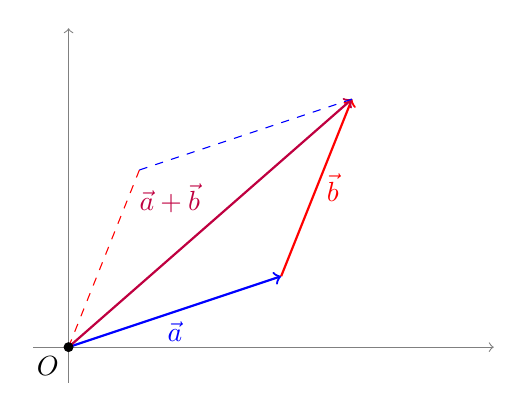
\begin{tikzpicture}[scale=0.9]
  \draw[->,gray] (-0.5,0) -- (6,0);
  \draw[->,gray] (0,-0.5) -- (0,4.5);
  \draw[->,thick,blue] (0,0) -- (3,1) node[midway,below] {$\vec{a}$};
  \draw[->,thick,red] (3,1) -- (4,3.5) node[midway,right] {$\vec{b}$};
  \draw[->,thick,purple] (0,0) -- (4,3.5) node[midway,above left] {$\vec{a}+\vec{b}$};
  \draw[dashed,red] (0,0) -- (1,2.5);
  \draw[dashed,blue] (1,2.5) -- (4,3.5);
  \fill (0,0) circle (2pt) node[below left] {$O$};
\end{tikzpicture}
\end{center}

With coordinates, addition is almost absurdly simple: add corresponding components.
\[
(3,1)+(1,2.5)=(3+1,\;1+2.5)=(4,3.5).
\]
Joining head to tail geometrically and adding components algebraically describe the same thing. Chapter 4's coordinate bridge is carrying traffic again.

Addition naturally leads to scaling: stretch an arrow to $2$ times its length, shrink it to half, or reverse its direction. This is scalar multiplication, written $2\vec{v}$, $\tfrac{1}{2}\vec{v}$, and $-\vec{v}$. In coordinates, multiply every component by the same number: $2\cdot(3,4)=(6,8)$.

Return to the game. Write $\vec{f}$ for one forward step and $\vec{l}$ for one leftward step. Your whole afternoon---$3$ steps forward, $2$ left, then turning around and taking $1$ forward---becomes
\[
3\vec{f}+2\vec{l}+(-1)\vec{f}=2\vec{f}+2\vec{l}.
\]
A travel diary has become one line of algebra. An expression like $3\vec{f}+2\vec{l}$, formed by multiplying vectors by numbers and adding, is a \textbf{linear combination}. Linear here means that we allow only addition and scalar multiplication, those two simplest operations, without multiplying vectors together, squaring them, or doing anything more elaborate. Do not underestimate the restriction: mathematics built from just these two operations is among the world's most powerful.

The next question determines the chapter's direction: which arrows should be our basic steps so that every possible movement in the plane is a linear combination of them?

One arrow is plainly insufficient: if you can only move forward, you can never reach a well to the side. What about two noncollinear arrows, such as $\vec{f}$ pointing east and $\vec{l}$ north? Intuitively, any movement can be divided into some amount east and some amount north. Two independent directions seem sufficient in the plane, while a $3$rd arrow, say northeast, is redundant because it is already a linear combination of the first two.

\begin{shuyu}{Basis and Dimension}
Intuition: a basis is a collection of basic steps, with too few leaving destinations unreachable and too many creating redundancy. The dimension counts those steps.

Formal definition: a collection of vectors is a basis of a space if it is linearly independent (none is a linear combination of the others) and its linear combinations fill the entire space. The number of vectors in a basis is the dimension of the space.

Example: $\vec{e}_1=(1,0)$ and $\vec{e}_2=(0,1)$ form a basis of the plane, which is two-dimensional. So do $(1,0)$ and $(1,1)$: a basis is not unique.
\end{shuyu}

Dimension, a word we have used casually for years, finally has a precise meaning: how many independent basic directions are minimally needed to assemble every vector? A line has one dimension, a plane two, and our physical space three. Algebra is untroubled by larger numbers: a list of a hundred components, $(x_1,x_2,\dots,x_{100})$, can still be added and scaled, and is a vector in a hundred-dimensional space. We can no longer draw the arrow, but the arithmetic works as usual. This is the title's passage to higher dimensions: algebraic rules carry two-dimensional intuition unchanged into places our eyes cannot see.

\section{The Central Theorem: Each Arrow Has Just One Expression}

Why believe that two independent arrows can assemble everything in the plane? Intuition is not enough. Let us make it a theorem and prove it.

\begin{dingli}[Uniqueness of Coordinates]
Let $\vec{e}_1$ and $\vec{e}_2$ be two noncollinear vectors in the plane. Every plane vector $\vec{v}$ can be written uniquely as
\[
\vec{v}=a\vec{e}_1+b\vec{e}_2,
\]
where $a$ and $b$ are real numbers. The representation always exists, and there is exactly one pair of coefficients.
\end{dingli}

\begin{proof}
First prove existence. Translate the tails of $\vec{e}_1$, $\vec{e}_2$, and $\vec{v}$ to a common point $O$. Through the tip of $\vec{v}$, draw a line parallel to $\vec{e}_2$, meeting the line containing $\vec{e}_1$ at $P$. Since $\vec{e}_1$ and $\vec{e}_2$ are noncollinear, these lines are not parallel and must meet. The arrow from $O$ to $P$ is collinear with $\vec{e}_1$, so it is some multiple $a\vec{e}_1$ of $\vec{e}_1$. The segment from $P$ to the tip of $\vec{v}$ is collinear with $\vec{e}_2$, so it is some multiple $b\vec{e}_2$. The triangle rule gives $\vec{v}=a\vec{e}_1+b\vec{e}_2$.

Now prove uniqueness. Suppose one arrow has two expressions:
\[
\vec{v}=a\vec{e}_1+b\vec{e}_2=a'\vec{e}_1+b'\vec{e}_2.
\]
Subtracting gives $(a-a')\vec{e}_1+(b-b')\vec{e}_2=\vec{0}$. If $a-a'\neq 0$, then
\[
\vec{e}_1=-\frac{b-b'}{a-a'}\,\vec{e}_2,
\]
which makes $\vec{e}_1$ a multiple of $\vec{e}_2$: the arrows would be collinear, contradicting the assumption. Thus $a=a'$, and similarly $b=b'$. There is just one representation.
\end{proof}

Pause to examine the theorem. Once a basis is chosen, every plane vector corresponds one to one with an ordered pair $(a,b)$ of real numbers. Vectors are geometrical objects and coordinates algebraic objects; the theorem guarantees a perfect translation, with nothing added or lost. In Chapter 4 we wrote $(x,y)$ every day while implicitly relying on this result. It has finally stepped out from backstage to receive a proof.

The same linear-combination viewpoint resolves a geometrical puzzle left from Chapter 2. What picture does the system
\[
\begin{cases}
2x+y=5,\\
x-y=1
\end{cases}
\]
draw? There are two views, both correct and important.

The first reads row by row: each equation is a line, and a solution is a shared point. Intersecting lines give one solution; distinct parallel lines give none; coincident lines give infinitely many. There are no other cases, because two plane lines have only these three relationships. Numerically, adding gives $3x=6$, so $x=2$; substitution gives $y=1$, and the intersection is $(2,1)$.

\begin{center}
\begin{tikzpicture}[scale=0.7]
  \draw[->,gray] (-1,0) -- (6,0) node[right] {$x$};
  \draw[->,gray] (0,-2) -- (0,5.5) node[above] {$y$};
  \draw[thick,blue] (-0.5,6) -- (3.5,-2) node[below right] {$2x+y=5$};
  \draw[thick,red] (0.5,-0.5) -- (5,4) node[above right] {$x-y=1$};
  \fill (2,1) circle (2.5pt) node[below right] {$(2,1)$};
\end{tikzpicture}
\end{center}

The second reads column by column, rewriting the system as
\[
x\begin{pmatrix}2\\1\end{pmatrix}+y\begin{pmatrix}1\\-1\end{pmatrix}=\begin{pmatrix}5\\1\end{pmatrix}.
\]
It asks which multiples of $(2,1)$ and $(1,-1)$ assemble the target arrow $(5,1)$. The solution is unique precisely because the two arrows are noncollinear: they form a basis, and the theorem guarantees one assembly. No solution corresponds to collinear arrows with the target off their line, unreachable by any combination. Infinitely many solutions correspond to all three arrows being collinear, allowing many combinations.

In three dimensions, each linear equation in three unknowns is a plane. Three planes may meet at one point (one solution), along a line (infinitely many), or pairwise like open book pages without a common point (no solution). Algebra's questions of existence and number of solutions become geometry's questions of how planes are arranged. Linear algebra is essentially the art of translating between these pictures.

\section{Matrices: Putting Transformations into Arrays}

Chapter 6 studied actions such as rotation, scaling, and reflection in geometrical language: rotate the entire plane $90^\circ$ about the origin, or multiply every distance from the origin by $2$. With vectors and coordinates, we can ask something practical: can every action have an instruction sheet into which we insert any point's coordinates and calculate its new coordinates?

Start with a $90^\circ$ anticlockwise rotation. Experiment on the basis arrows: $\vec{e}_1=(1,0)$ goes to $(0,1)$, and $\vec{e}_2=(0,1)$ goes to $(-1,0)$. By uniqueness of coordinates, an arbitrary vector $(x,y)=x\vec{e}_1+y\vec{e}_2$ becomes
\[
x\cdot(0,1)+y\cdot(-1,0)=(-y,\;x).
\]
Check a specific point: $(3,1)$ should become $(-1,3)$. Draw it on squared paper: the length is unchanged and the direction has turned one right angle anticlockwise.

Place the two images $(0,1)$ and $(-1,0)$ side by side as columns in an array:
\[
A=\begin{pmatrix}0&-1\\1&0\end{pmatrix}.
\]
This array is a matrix. Define multiplication of $A$ by a vector $(x,y)$ using the row-times-column rule:
\[
\begin{pmatrix}0&-1\\1&0\end{pmatrix}\begin{pmatrix}x\\y\end{pmatrix}
=\begin{pmatrix}0\cdot x+(-1)\cdot y\\1\cdot x+0\cdot y\end{pmatrix}
=\begin{pmatrix}-y\\x\end{pmatrix}.
\]
The first row computes the first output component, and the second row the second. A rotation of the entire plane has been compressed into four numbers.

Now scale every distance from the origin by $2$. The direction of $\vec{e}_1$ stays fixed as it lengthens to $(2,0)$, and $\vec{e}_2$ becomes $(0,2)$. The matrix is
\[
\begin{pmatrix}2&0\\0&2\end{pmatrix},
\]
which takes $(x,y)$ to $(2x,2y)$. Similarly, reflection in the $x$-axis is $\begin{pmatrix}1&0\\0&-1\end{pmatrix}$, and a horizontal shear is $\begin{pmatrix}1&1\\0&1\end{pmatrix}$.

Why can matrices hold these transformations? Rotations, scalings, reflections, and shears share a helpful temperament: they take lines to lines, fix the origin, and satisfy
\[
T(\vec{u}+\vec{v})=T(\vec{u})+T(\vec{v}),\qquad T(c\vec{v})=c\,T(\vec{v}).
\]
A transformation with these two properties is \textbf{linear}. Their power is that once we know the destinations of two basis arrows, the destination of any vector $x\vec{e}_1+y\vec{e}_2$ is forced: its image must be the same linear combination of the basis images. Thus all information about a linear transformation is concentrated in the two basis images, the matrix's two columns. A matrix is a complete record of a transformation, not an arbitrary arrangement of numbers.

What about successive actions? Rotate $90^\circ$ and then scale by $2$. The combined matrix is exactly the product of the two matrices under the row-times-column rule. Calculate it explicitly:
\[
\begin{pmatrix}2&0\\0&2\end{pmatrix}\begin{pmatrix}0&-1\\1&0\end{pmatrix}
=\begin{pmatrix}2\cdot0+0\cdot1&2\cdot(-1)+0\cdot0\\0\cdot0+2\cdot1&0\cdot(-1)+2\cdot0\end{pmatrix}
=\begin{pmatrix}0&-2\\2&0\end{pmatrix}.
\]
Check $(3,1)$: rotate $90^\circ$ to get $(-1,3)$, then scale by $2$ to get $(-2,6)$. Applying the product directly gives $(0\cdot3+(-2)\cdot1,\;2\cdot3+0\cdot1)=(-2,6)$, exactly the same. Watch the order, though. Scaling then rotating gives the same product here because these two transformations happen to commute. But rotating then reflecting and reflecting then rotating generally differ. Matrix multiplication is not always commutative, matching the importance of action order already seen in Chapter 6's discussion of the cube.

Chapter 6's composition was a geometrical operation; matrix multiplication is its shadow in coordinates. Your game character turning, the camera zooming, and a three-dimensional model appearing on screen all involve chains of matrix products. Much of a graphics chip's work every second is simply very fast matrix multiplication.

\begin{lianjie}
Looking back, Chapter 4 used numbers to describe points, and this chapter uses arrays to describe transformations: the same bridge has grown wider. Chapter 6's rotations and reflections have become explicit arrays, and the square's eight symmetries correspond to eight $2\times2$ matrices. Looking ahead, in Chapter 8 vectors and matrices will describe the line that a curve resembles near a point. In secondary school and university they will appear in physical forces and velocities, economic input-output models, and every frame of computer graphics. Linear algebra is a common native language of science and engineering.
\end{lianjie}

\section{Arrows That Keep Their Direction: Eigenvectors}

A typical linear transformation turns most arrows in new directions. A $90^\circ$ rotation is extreme: no arrow retains its original direction. But some transformations hide loyal arrows whose direction stays the same, or reverses exactly, while only their length changes.

Consider a specific example:
\[
M=\begin{pmatrix}2&1\\1&2\end{pmatrix}.
\]
Try a few arrows. $(1,0)$ goes to $(2,1)$, changing direction; $(0,1)$ goes to $(1,2)$, also changing direction. But $(1,1)$ goes to
\[
\begin{pmatrix}2&1\\1&2\end{pmatrix}\begin{pmatrix}1\\1\end{pmatrix}=\begin{pmatrix}3\\3\end{pmatrix}=3\begin{pmatrix}1\\1\end{pmatrix},
\]
keeping its direction exactly and growing by a factor of $3$! Now examine $(1,-1)$, along the northwest--southeast direction. Perhaps the transformation treats it more gently. Calculation gives
\[
\begin{pmatrix}2&1\\1&2\end{pmatrix}\begin{pmatrix}1\\-1\end{pmatrix}=\begin{pmatrix}1\\-1\end{pmatrix},
\]
with both direction and length unchanged.

\begin{shuyu}{Eigenvectors and Eigenvalues}
Intuition: an arrow that a transformation does not turn aside. It keeps its direction or reverses, and is merely stretched, shortened, or left alone.

Formal definition: for a matrix $A$, if a nonzero vector $\vec{v}$ satisfies $A\vec{v}=\lambda\vec{v}$ for some number $\lambda$, then $\vec{v}$ is an eigenvector of $A$, with corresponding eigenvalue $\lambda$.

Example: the matrix $M$ above has eigenvector $(1,1)$ with eigenvalue $3$, and eigenvector $(1,-1)$ with eigenvalue $1$.
\end{shuyu}

Why find these arrows? Eigenvectors are the transformation's principal axes. Along them, a complicated transformation reduces to the simplest action: stretching or shrinking. The matrix $M$ seems to mix up the plane, but it merely stretches the northeast--southwest direction by $3$ and leaves the northwest--southeast direction unchanged. Understand those two axes and you understand the whole transformation. Mathematicians often say that the best way to understand a linear transformation is to find all its eigenvectors, like taking a photograph of its skeleton.

\section{Another Perspective: Compression, Ranking, and Vibration}

Linear algebra sounds abstract, yet it hides in three things you use every day.

\textbf{Image compression.} A grayscale photograph with $512\times512$ pixels is essentially a $512\times512$ matrix, with each entry recording brightness. Direct storage requires more than $26$ times ten thousand numbers. But a photograph is not random: the sky's values are almost identical, and a wall corner changes sharply in only a few directions. Linear algebra offers singular value decomposition, splitting the matrix into a sum of characteristic directions, with the most important few carrying over ninety percent of the visual information. Keep only the first few dozen and discard the rest, and the data may shrink to a tenth while the eye notices little difference. Every JPEG on your phone and every streamed animated episode relies on this kind of idea: approximating a whole matrix through a few important directions.

\textbf{Web ranking.} Imagine the Internet as a giant network: every page is a point and every link an arrow. How does a search engine judge importance? An ingenious idea gives each page an importance score equal to the sum of contributions from pages linking to it. Being cited by more important pages makes a page more important. Try a toy Internet of three pages: page A is cited by B and C, B by C, and C by A. Give them scores $x$, $y$, and $z$. The rules say that $x$ receives contributions from B and C, $y$ from C, and $z$ from A: three unknowns and three equations. Arrange the scores as a three-dimensional vector $\vec{v}=(x,y,z)$ and the link rules in a $3\times3$ matrix $A$, and the equation is exactly $A\vec{v}=\vec{v}$.

Replace the toy with the real Internet, and tens of billions of pages mean tens of billions of unknowns. Frightening? It is still a linear system, specifically the problem of finding an eigenvector of a huge matrix. The score vector satisfies $A\vec{v}=\vec{v}$, so it is an eigenvector with eigenvalue $1$. In practice, we avoid solving directly and use the trick in Experiment 2: begin with guessed scores and multiply repeatedly by $A$. The vector with billions of dimensions quickly leans toward the most important eigenvector, establishing the ranking. At the heart of one of the world's most profitable algorithms lies this chapter's equation $A\vec{v}=\lambda\vec{v}$.

\textbf{Vibration.} Pluck a guitar string fixed at both ends and it vibrates to make sound. Its constantly changing shape seems complicated, but physicists discovered that every vibration can be decomposed into standard modes: the low fundamental tone, the overtone an octave above, and so on. Each standard mode is an eigenvector of the string's equation of motion, and its eigenvalue determines the pitch. A string's rich tone is many eigenmodes singing together. Earthquake-resistant buildings, bridge design, and microphone noise reduction all use the same analysis: break complicated motion into simple motions along characteristic directions.

\begin{toolbox}
This chapter's new tools:
\begin{itemize}
\item Vectors: an arrow, or coordinate pair, records magnitude and direction together. Addition joins head to tail geometrically and adds components algebraically.
\item Linear combinations and bases: every vector is a linear combination of basis vectors with unique coefficients, making coordinates reliable.
\item Dimension: the minimum number of independent directions needed to fill a space; the same rules work in a hundred dimensions.
\item Matrices: complete records of linear transformations, with two columns giving the images of two basis arrows. Matrix multiplication corresponds to composition.
\item The geometry of systems: intersections of lines and planes express the problem of assembling a target arrow from basis arrows.
\item Eigenvectors: arrows retaining their direction reveal a transformation's principal axes, the common heart of compression, ranking, and vibration analysis.
\end{itemize}
\end{toolbox}

\begin{shiyan}
\textbf{Experiment 1: Building with Basis Arrows.} On squared paper, use $\vec{e}_1=(2,1)$ and $\vec{e}_2=(-1,2)$ as basis arrows. Assemble $\vec{v}=(1,8)$ by finding $a\vec{e}_1+b\vec{e}_2=\vec{v}$, or solving $2a-b=1$ and $a+2b=8$. Calculate, then draw the triangle rule to check. Replace the basis with the collinear arrows $(2,1)$ and $(4,2)$ and try to assemble $(1,8)$ again. Experience how collinearity leaves a direction missing.

\textbf{Experiment 2: Following an Arrow's Fate.} Take $M=\begin{pmatrix}2&1\\1&2\end{pmatrix}$. Draw $(1,0)$, $(1,1)$, $(1,-1)$, and $(2,1)$, calculate their images under $M$, and draw them too. Which arrows keep their direction? Which stretches most? Apply $M$ three times successively to $(1,0)$ and watch the direction it increasingly approaches: the eigenvector with the largest eigenvalue. This is how web-ranking algorithms actually compute an eigenvector: repeated multiplication lets the most important direction emerge.
\end{shiyan}

\begin{pandeng}
For further climbing, look for these terms: determinants, measuring area scaling and detecting whether a basis degenerates; inverse matrices, instructions for undoing transformations; computing eigenvalues through the characteristic equation; singular value decomposition, the main character in image compression; Markov chains, the probabilistic clothing of web ranking; and vector spaces and Hilbert spaces, extending vectors to functions and providing a home for Fourier series. Competition topics such as the fundamental theorem of plane vectors and points dividing segments in a given ratio are direct descendants of this chapter's story.
\end{pandeng}

\section*{Questions to Think About}

\textbf{Observation}

1. Draw any three arrows $\vec{a}$, $\vec{b}$, and $\vec{c}$ on squared paper. Use the triangle rule to draw $(\vec{a}+\vec{b})+\vec{c}$ and $\vec{a}+(\vec{b}+\vec{c})$. What do you observe? Now compare $\vec{a}+\vec{b}$ and $\vec{b}+\vec{a}$. (Hint: carry out every addition head to tail, rather than trusting a visual impression.)

2. For the horizontal shear $\begin{pmatrix}1&1\\0&1\end{pmatrix}$, calculate the images of the $x$-axis arrow $(1,0)$ and the $y$-axis arrow $(0,1)$. Are there eigenvectors? (Hint: an arrow keeps its direction only if its two components scale by the same factor.)

\textbf{Proof}

1. Prove that if $\vec{v}_1$ and $\vec{v}_2$ are eigenvectors of $A$ with eigenvalue $\lambda$, every nonzero linear combination $a\vec{v}_1+b\vec{v}_2$ is also an eigenvector with eigenvalue $\lambda$. (Hint: start from $A\vec{v}_1=\lambda\vec{v}_1$ and $A\vec{v}_2=\lambda\vec{v}_2$, and apply the two linearity properties to $A(a\vec{v}_1+b\vec{v}_2)$.)

2. Prove that anticlockwise rotation through $\theta$ about the origin has matrix $\begin{pmatrix}\cos\theta&-\sin\theta\\ \sin\theta&\cos\theta\end{pmatrix}$. (Hint: calculate only the images of $(1,0)$ and $(0,1)$; these are the columns. Recall the meanings of $\cos$ and $\sin$ from coordinates on the unit circle.)

\textbf{Challenge}

1. Can you find arrangements of three planes that intersect pairwise without a shared point, besides the open-book picture mentioned in the text? What algebraic reason for inconsistency corresponds to each arrangement? (Hint: intersect the first two planes in a line, then consider the third plane's possible relationships with that line.)

2. Let $A$ act repeatedly on the plane: $\vec{v}_0=(1,0)$ and $\vec{v}_{n+1}=A\vec{v}_n$. For $A=\begin{pmatrix}2&1\\1&2\end{pmatrix}$, calculate $\vec{v}_1$ through $\vec{v}_4$. Which arrow does the direction of $\vec{v}_n$ approach, and approximately what factor multiplies its length at each step? Can you explain why repeated multiplication by the same matrix always draws an arrow toward the eigenvector with largest eigenvalue? (Hint: express $\vec{v}_0$ as a linear combination of the two eigenvectors and count how often each term is multiplied by $3$ or by $1$.)

\section*{The Door to the Next Chapter}

This chapter lived in a straight world: vectors were straight arrows, matrices sent lines to lines, and systems were solved at intersections of lines and planes. Linear algebra is powerful precisely because straight lines are the easiest geometrical objects to understand completely.

But the world is not always straight. Roller-coaster tracks bend, the water surface in a coffee cup curves, and Earth's surface is curved. Does a curved track still have a direction? Can an arrow sit on a sphere? Can a number measure where the bending is sharpest?

The mathematicians' answer fits this chapter's spirit surprisingly well. Curved objects may be complicated as wholes, but magnify enough and look locally enough, and each small piece is approximately straight. Near each point of a bend lies a line that best follows it; near each point of a surface lies a plane that best fits it. Lines and planes are exactly the objects we have just mastered. Next chapter, we will ask why a tiny part of a curve resembles a line and extend our linear world across the curved one.
